\documentclass[a4paper, 14pt]{article}				% general format

\usepackage[utf8]{inputenc}					% accept different input encodings
\usepackage[russian]{babel}					% multilingual support (T2A)
\usepackage{graphicx}
\usepackage{float}
\usepackage{amsmath}
\usepackage[boxed]{algorithm2e}
\usepackage{url}
\usepackage{fancyvrb}
\usepackage[dvipsnames]{xcolor}

\usepackage{listings}						% typeset source code listings

% Цвета для кода
\definecolor{string}{HTML}{101AF9}			% цвет строк в коде
\definecolor{comment}{HTML}{3F7F5F}		% цвет комментариев в коде
\definecolor{keyword}{HTML}{5F1441}			% цвет ключевых слов в коде
\definecolor{morecomment}{HTML}{8000FF}		% цвет include и других элементов в коде
\definecolor{captiontext}{HTML}{FFFFFF}		% цвет текста заголовка в коде
\definecolor{captionbk}{HTML}{999999}		% цвет фона заголовка в коде
\definecolor{bk}{HTML}{FFFFFF}			% цвет фона в коде
\definecolor{frame}{HTML}{999999}			% цвет рамки в коде

% Настройки отображения кода
\lstset{
	language=C++,						% Язык кода по умолчанию
	% Цвета
	keywordstyle=\color{keyword}\ttfamily\bfseries,
	stringstyle=\color{string}\ttfamily,
	commentstyle=\color{comment}\ttfamily\itshape,
	morecomment=[l][\color{morecomment}]{\#},
	% Настройки отображения
	breaklines=true,					% Перенос длинных строк
	basicstyle=\ttfamily\footnotesize,		% Шрифт для отображения кода
	backgroundcolor=\color{bk},			% Цвет фона кода
	frame=tblr						% draw a frame at all sides of the code block
	rulecolor=\color{frame},				% Цвет рамки
	tabsize=2,						% tab space width
	showstringspaces=false,				% don't mark spaces in strings
	% Настройка отображения номеров строк. Если не нужно, то удалите весь блок
	numbers=left,					% Слева отображаются номера строк
	stepnumber=1,					% Каждую строку нумеровать
	numbersep=5pt,					% Отступ от кода
	numberstyle=\small\color{black},			% Стиль написания номеров строк
	}
% Для настройки заголовка кода
\usepackage{caption}
\DeclareCaptionFont{white}{\color{сaptiontext}}
\DeclareCaptionFormat{listing}{\parbox{\linewidth}{\colorbox{сaptionbk}{\parbox{\linewidth}{#1#2#3}}\vskip-4pt}}
%\captionsetup[lstlisting]{format=listing,labelfont=white,textfont=white}
\renewcommand{\lstlistingname}{Листинг} % Переименование Listings в нужное именование структуры

\author{Певцов Игорь, гр.53501/3}
\title{Отчет по лабораторной работе 7:\\"Сервис тестирования корректности настройки SSL на сервере Qualys SSL Labs – SSL Server Test"\\ по дисциплине\\"Методы и средства защиты информации"}

\begin{document}
\maketitle

\newpage
\tableofcontents{}

\newpage
\section{Цель работы}
Изучить сервис тестирования корректности настройки SSL на сервере Qualys SSL Labs и его основные возможности.
\section{Ход работы}
\subsection{Изучение}
\subsubsection{Лучшие практики по развертыванию SSL}
\begin{itemize}
\item Использовать 2048-битные закрытые ключи.
Использовать 2048-битный RSA или 256-битные ECDSA закрытые ключи для всех серверов. Ключи такой крепости безопасны и будут оставаться безопасными в течение значительного периода времени.
\item Защитить закрытый ключ. Предоставить доступ к ключу как можно меньшей группе сотрудников.
\item Обеспечить охват всех используемых доменных имен. Убедиться, что сертификаты охватывают все доменные имена, которые используются на сайте.
\item Приобретать сертификаты у надежного CA.
\item Использовать надежные алгоритмы подписи сертификата. Безопасность сертификата зависит от длины закрытого ключа и прочности используемой функции хеширования. Сегодня большинство сертификатов используют алгоритм SHA1, который считается слабым. 
\item Использовать безопасные протоколы. (TLS v1.0/v1.1/v1.2)
\item Использовать безопасные алгоритмы шифрования. В данном случае подойдут симметричные алгоритмы с ключами более 128 бит.
\item Контролировать выбор алгоритма шифрования. В SSL версии 3 и более поздних версиях протокола, клиенты отправляют список алгоритмов шифрования, которые они поддерживают, и сервер выбирает один из них для организации безопасного канала связи. Не все сервера могут делать это хорошо, так как некоторые выбирают первый поддерживаемый алгоритм из списка.
\item Использование Forward Secrecy. Forward Secrecy — это особенность протокола, который обеспечивает безопасный обмен данными, он не зависит от закрытого ключа сервера. С алгоритмами шифрования, которые не поддерживают Forward Secrecy, возможно расшифровать ранее зашифрованные разговоры с помощью закрытого ключа сервера.
\item Отключить проверку защищенности по инициативе клиента.
\end{itemize}

\subsubsection{Основные уязвимости и атаки на SSL последнего времени - POODLE, HeartBleed}
\paragraph {POODLE\\}
Атака POODLE(Padding Oracle On Downgraded Legacy Encryption) работает по следующему сценарию: Взломщик отправляет свои данные на вервер по протоколу SSL3 от имени взламываемой структуры, что позволяет ему постепенно расшифровывать данные из запросов. Это возможно, так как в SSL3 нету привязки к MAC адресу.

\paragraph {Heartbleed\\}
Ошибка (переполнение буфера) в криптографическом программном обеспечении OpenSSL, позволяющая несанкционированно читать память на сервере или на клиенте, в том числе для извлечения закрытого ключа сервера. Информация об уязвимости была опубликована в апреле 2014 года, ошибка существовала с конца 2011 года.
\begin{figure}[h!]
\centering
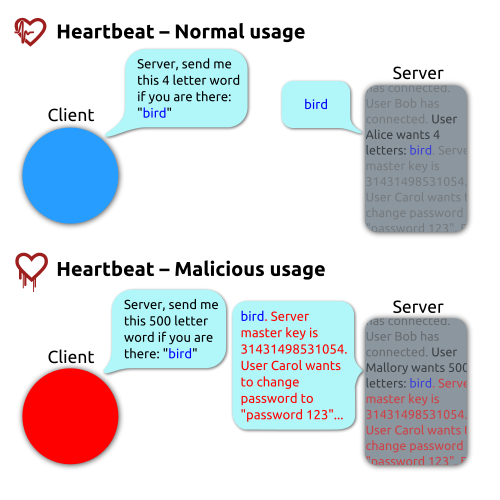
\includegraphics[width=\textwidth]{rsrc/lab7_heartbleed}
\caption{Принцип работы heartbleed.}
\end{figure}
\subsection{Выбрать со стартовой страницы SSL Server Test один домен из списка Recent Best и один домен из списка Recent Worst, интерпретировать результаты в разделе Summary}
\paragraph {Recent Best\\}
\begin{figure}[h!]
\centering
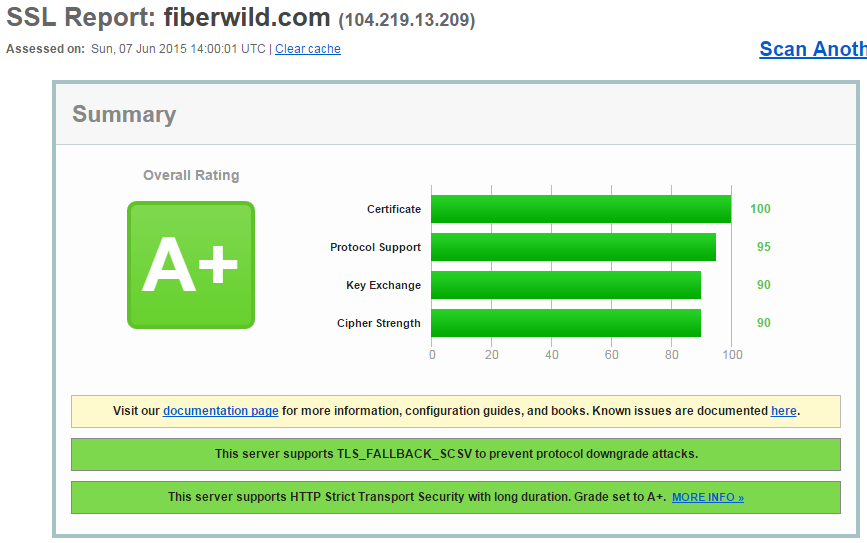
\includegraphics[width=\textwidth]{rsrc/lab7_best}
\caption{Раздел Summary для Recent Best.}
\end{figure}
\begin{itemize}
\item{Поддерживаются все версии протокола TLS.}
\item{Поддерживается заголовок HTTP Strict Transport Security на протяжении длительного времени.}
\item{Защита от downgrade-атак.}
\end{itemize}

\newpage
\paragraph {Recent Worst\\}
\begin{figure}[h!]
\centering
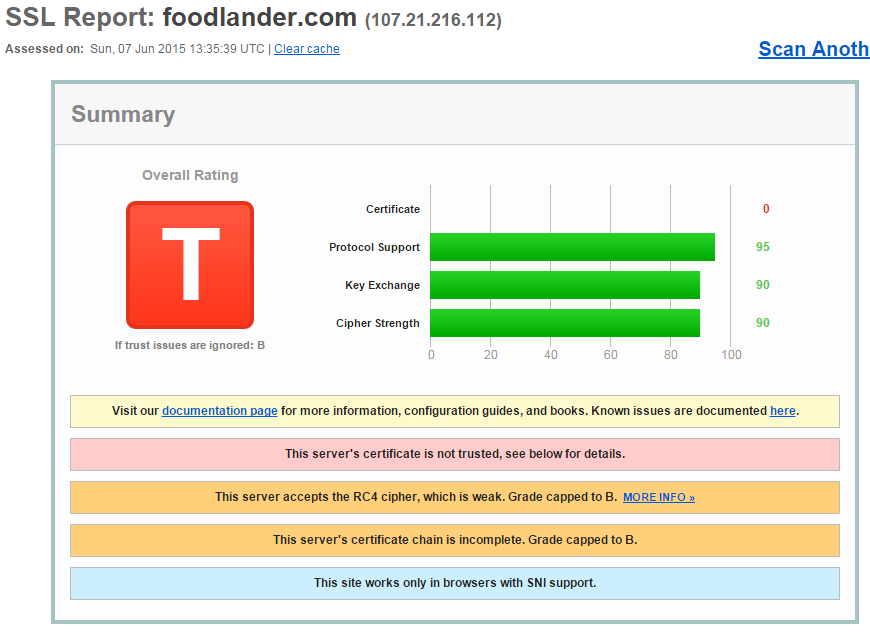
\includegraphics[width=\textwidth]{rsrc/lab7_worst}
\caption{Раздел Summary для Recent Worst.}
\end{figure}

\begin{itemize}
\item{Сертификат не подписан.}
\item{Сервер позволяет использовать слабый шифр RC4.}
\item{Цепочка сертификации сервера неполная.}
\item{Сайт работает только в браузерах, которые поддерживают SNI(Server Name Indication) - расширение к протоколу TLS}
\end{itemize}

\newpage
\subsection{Выбор интернет-домена, защищенного SSL-шифрованием.}
В качестве испытуемого был выбран домен fwallet.tk, над которым мы работали в курсе ТРПО. На домене развернут стандартный набор LAMP, а также используется бесплатный SSL сертификат от WoSign.\\

\paragraph{Summary\\}
\begin{figure}[h!]
\centering
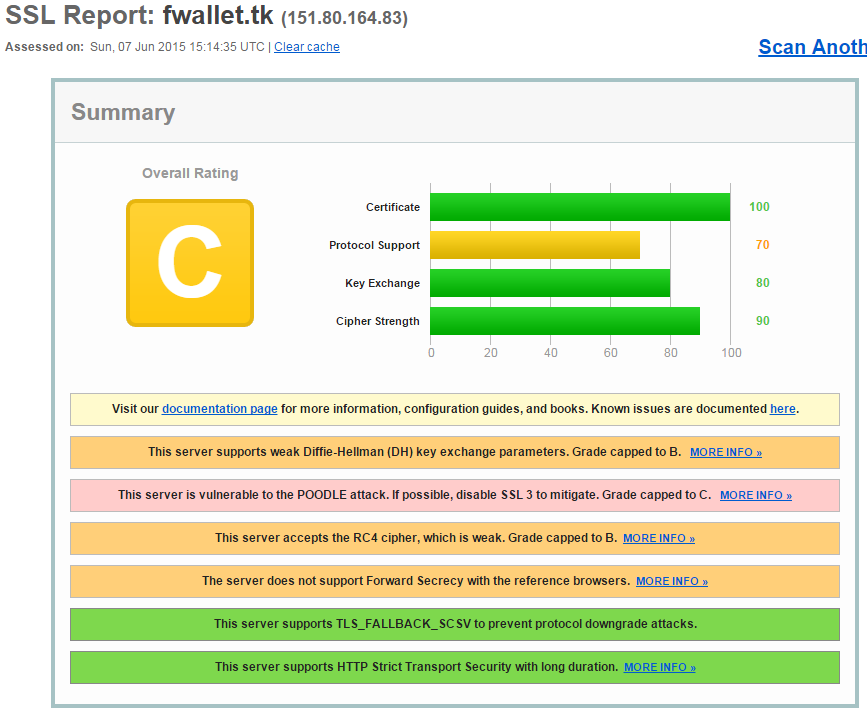
\includegraphics[width=\textwidth]{rsrc/lab7_fw_sum}
\caption{Раздел Summary для Recent Worst.}
\end{figure}
\begin{itemize}
\item{(-) Сервер подерживает слабую версию алгоритма Диффи-Хеллмана обмена ключами.}
\item{(-) Сервер уязвим к атакам POODLE.}
\item{(-) Сервер позволяет использовать слабый шифр RC4.}
\item{(-) Сервер не поддерживает Forward Secrecy}
\item{(+) Защита от downgrade-атак.}
\item{(+) Поддерживается заголовок HTTP Strict Transport Security на протяжении длительного времени.}
\end{itemize}

\paragraph{Configuration\\}
\begin{figure}[h!]
\centering
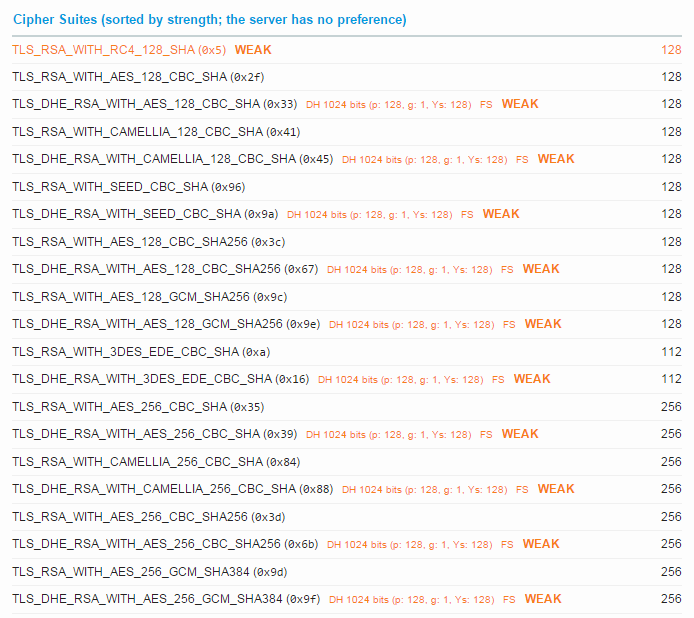
\includegraphics[width=\textwidth]{rsrc/lab7_fw_conf}
\caption{Раздел Summary для Recent Worst.}
\end{figure}
\begin{itemize}
\item{Все шифры, испльзующие DHE(Diffie-Hellman Exchange) помечены как WEAK(слабые).}
\item{RSA - Rivest, Shamir, Adleman - криптографический алгоритм}
\item{RC4 - Rivest Cipher 4 -  потоковый шифр 4-й версии}
\item{SHA/SHA256/384 - Secure Hash Algorithm - Алгоритм хэширования. Цифра - длина ключа}
\item{AES - Advanced Encryption Standard - симметричный алгоритм блочного шифрования}
\item{GCM и CBC это два режима блочного шифрования}
\item{TLS - Transport Layer Security - криптографический протокол}
\item{3DES - Digital Encryption Standard - алгоритм блочного шифрования}
\item{EDE - Encrypt, Decrypt, Encrypt - режим работы алгоритма 3DES}
\item{Camellia - симметричный алгоритм блочного шифрования}
\end{itemize}

\paragraph{Protocol details\\}
\begin{figure}[h!]
\centering
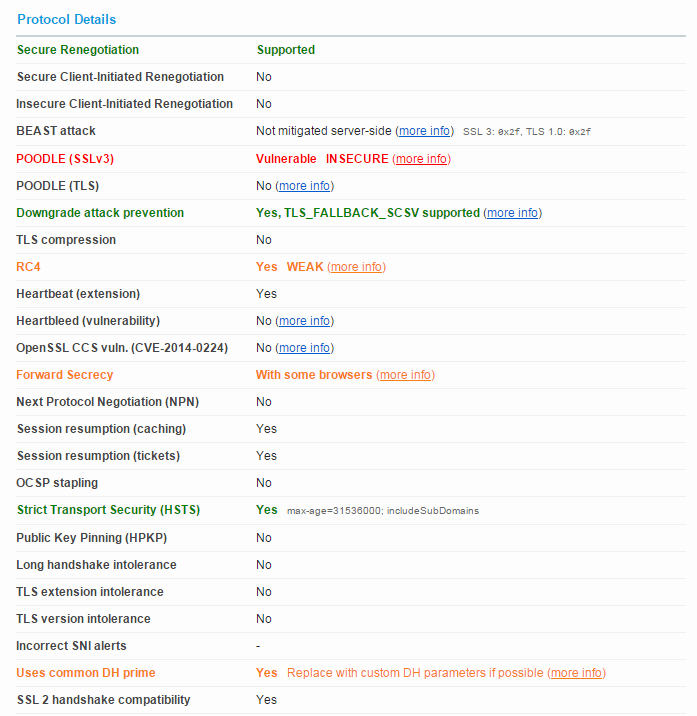
\includegraphics[width=\textwidth]{rsrc/lab7_fw_prot}
\caption{Раздел Summary для Recent Worst.}
\end{figure}

\begin{itemize}
\item{Строки 1-3 - перепроверка сертификата и защищенность этого процесса, все в порядке.}
\item{Строки 4-7 - Проверка уязвимости к атакам BEAST, POODLE, downgrade. Система уязвима к POODLE SSLv3}
\item{Строки 8 - сжатие TLS не используется}
\item{Строка 9 - Используется слабый шифр RC4}
\item{Строки 10-12 - уязвимости OpenSSL Heartbleed, etc.}
\item{Строка 13 - совместимость Forward Secrecy с новыми браузерами.}
\item{Строки 15-16 - Поддерживает возобновление сессии с помощью частичного хэндшейка}
\item{Строка 18 - Поддерживает заголовки HSTS}
\item{Строка 19 - Не поддерживает заголовок HPKP - ассоциацию сервера с ключом}
\item{Строка 24 - Используются стандартные параметры для алгоритма Диффи-Хеллмана.}
\item{Строка 25 - Совместим с SSL 2 handshake}
\end{itemize}

\subsection{Сделать итоговый вывод о реализации SSL на заданном домене}
Подводя итог, можно сказать, что сервер защищен достаточно слабо, поскольку имеется критическая уязвимость к POODLE,  а также используется слабый шифр RC4, что может привести к расшифровке трафика. С сертификатом проблем не обнаружено, значит в подлинности сервера сомневаться не приходится. Сервер поддерживает восстановление TLS-сессии при помощи неполного хэндшейка, что существенно сокращает потребление процессорного времени и ускоряет работу. Forward Secrecy поддерживается только для новых браузеров, что впринципе не является проблемой.

\section{Выводы}
В результате выполнения данной лабораторной работы были изучены возможности веб-сервиса Qualys SSL LABS. Сервис позволяет получить развернутую статистику по SSL для запрашиваемого домена. Анализируя данные, полученные таким способом, можно значительно улучшить стабильность и безопасность сервера, закрыв все явные уязвимости.
\end{document}